% ltex: language=it
\chapter{Reti Neurali}\label{chap:reti_neurali} % (fold)
\section{Neuroni Biologici}\label{sec:neuroni_biologici} % (fold)
\begin{cimage}
    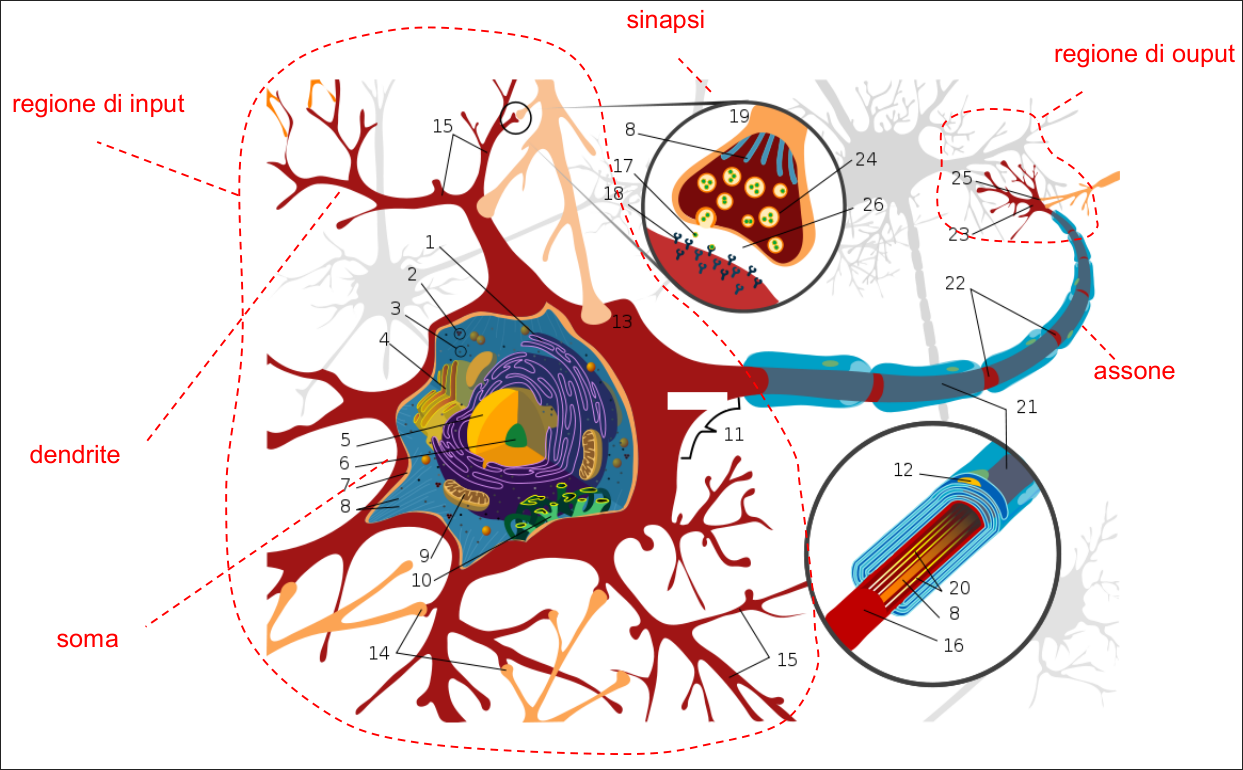
\includegraphics[width=.8\textwidth]{assets/bio-neuro.png}
\end{cimage}
I neuroni sono le più importanti \red{cellule} del sistema nervoso.
Le connessioni \textbf{sinaptiche}, o \textbf{sinapsi}, agiscono come porte di collegamento per il passaggio delle informazioni tra neuroni.
\\
I \textbf{dendriti} sono fibre minori che si ramificano a partire dal corpo cellulare del neurone, detto \textbf{soma}.
Attraverso le sinapsi i dendriti raccolgono \textbf{input} da neuroni afferenti e li propagano verso il soma.
\\
L'\textbf{assone} è la fibra principale che parte dal soma e si allontana da esso per portare ad altri neuroni l'\textbf{output}.
\begin{cimage}
    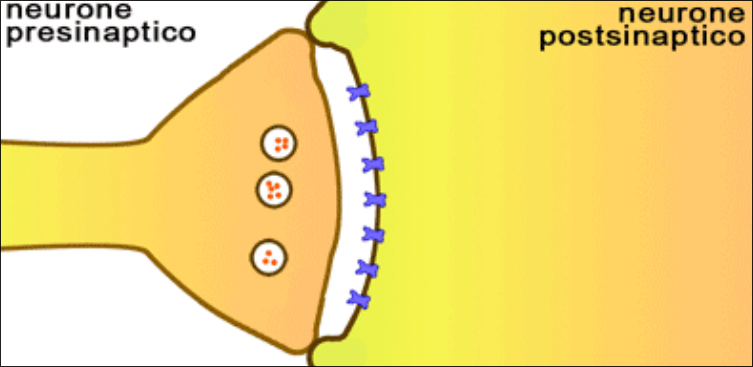
\includegraphics[width=.6\textwidth]{assets/pre-neu-post-visual.png}
\end{cimage}
Il passaggio delle informazioni avviene attraverso le sinapsi, avviene con processi \red{elettro-chimici}.
Il neurone presinaptico libera le sostanza (neurotrasmettitori) che attraverso il breve gap sinaptico e sono captati da appositi recettori, canali ionici, posizionati sulla membrana del neurone postsinaptico.
\\
L'ingresso di \textbf{ioni} attraverso i canali ionici determina la formazione di una differenza di potenziale tra il corpo del neurone postsinaptico e l'esterno.
Quando questo potenziale supera una certa soglia si produce un impulso, chiamato \textbf{spike}: il neurone propaga un breve segnale elettrico detto \textbf{potenziale d'azione} lungo il proprio assone; questo potenziale determina il rilascio di neurotrasmettitori dalle sinapsi dell'assone.
\emptyln{}
Il \textbf{reweighting} delle sinapsi, ovvero la modifica della loro efficacia di trasmissione, è direttamente collegato ai processi di apprendimento e memoria in accordo con la regola di Hebb.
\begin{note}[Hebbian Rule]
    Se due neuroni, tra loro connessi da una o più sinapsi, sono ripetutamente attivati simultaneamente allora le sinapsi che li connettono sono rinforzate
\end{note}
%
% section Neuroni Biologici (end)
\section{Neurone Artificiale}\label{sec:neurone_artificiale} % (fold)
\begin{cimage}
    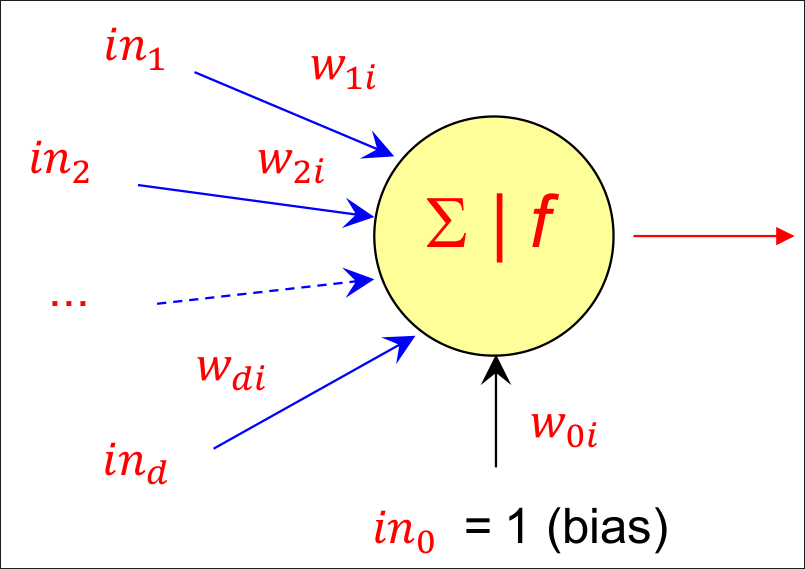
\includegraphics[width=.6\textwidth]{assets/art-neuro-visual.png}
\end{cimage}
\[
    \begin{aligned}
        net_i = &\sum_{\for[j][][d]}w_{ji}\cdot in_j + w_{0i} \\
        &out_i = f\pt{net_i}
    \end{aligned}
\]
\begin{itemize}
    \item $\vc{in_1}{in_d}$ sono i $d$ ingressi che il neurone $i$ riceve da assoni di neuroni afferenti;
    \item $\vc{w_{1i}}{w_{di}}$ sono i pesi, \red{weight}, che determinano l'efficacia delle connessioni sinaptiche dei dendriti (durante l'addestramento si manipolano questi valori);
    \item $w_{0i}$, detto \red{bias}, è un ulteriore peso che si considera collegato a un input fittizio con valore sempre $1$; questo è utile per <<tarare>> il punto di lavoro ottimale del neurone;
    \item $net_i$ è il \red{livello di eccitazione} globale del neurone (potenziale interno);
    \item $f\pt \cdot$ è la \red{funzione di attivazione} che determina il comportamento del neurone, ovvero il suo $out_i$ in funzione del suo livello di eccitazione $net_i$;
\end{itemize}
%
\subsection{Funzione di Attivazione}\label{sub:neur_funzione_di_attivazione} % (fold)
Nei neuroni biologici $f\pt \cdot$ è una funzione tutto-niente temporizzata: quanto $net_i$ supera una \textbf{certa soglia}, il neurone <<spara>> uno spike per poi tornare a riposo.
\begin{quote}
    Esistono reti artificiali, denominate \textbf{spiral neural network} che modellano questo comportamento e processano l'informazione attraverso treni di impulsi.
\end{quote}
Le reti neurali più comunemente utilizzate operano con \textbf{livelli continui} e $f\pt\cdot$ è una funzione \textbf{non-lineare} ma \textbf{continua} e \textbf{differenziabile}.
\\
Una delle funzioni di attivazione più comunemente utilizzata è la \textbf{sigmoide} nelle varianti:
\begin{itemize}
    \item \textbf{standard logistic function}, chiamata semplicemente sigmoid, con valori in $\itc{0,\,1}$:
        \[
            \fx[net] = \si\pt{net} = \frac{1}{1 + e^{-net}}
        \]
        La cui derivata è pari a:
        \[
            \sigma'\pt{net} = \frac{\dd}{\dd net}\pt{\frac{1}{1 + e^{-net}}} = \frac{e^{-net}}{\pt{1 + e^{-net}}^2} = \si\pt{net}\pt{1- \si\pt{net}}
        \]
    \item \textbf{tangente iperbolica} ($\tanh$) con valori in $\itc{-1,\,1}$: può essere ottenuta dalla funzione precedente, a seguito di una trasformazione di scala ($\times 2$) e traslazione ($-1$).
        \[
            \fx[net] = \tau\pt{net} = 2\si\pt{2 \cdot net} - 1
        \]
        La cui derivata è pari a:
        \[
            \tau'\pt{net} = 1 - \tau\pt{net}^2
        \]
        $\tanh$ è leggermente più complessa di sigmoid ma \red{preferibile} sia perché è simmetrica rispetto allo zero, sia perché converge più rapidamente;
\end{itemize}
% subsection Funzione di Attivazione (end)
% section Neurone Artificiale (end)
%
\section{Tipologie di Reti Neurali}\label{sec:tipologie_di_reti_neurali} % (fold)
Le reti neurali sono composte da gruppi di neuroni artificiali organizzati in livelli.
Tipicamente sono presenti: un livello di \textbf{input}, un livello di \textbf{output} e uno o più livelli \textbf{intermedi} o \textbf{nascosti}.
\begin{quote}
    Ogni livello contiene uno o più neuroni
\end{quote}
\begin{note}[Feedforward]
    Nelle reti \textbf{feedforward} le connessioni collegano i neuroni di un livello con i neuroni di un livello \red{successivo}.
    Non sono consentite connessioni all'indietro o connessioni verso lo stesso livello.
    È di gran lunga la rete più utilizzata.
    \begin{center}
        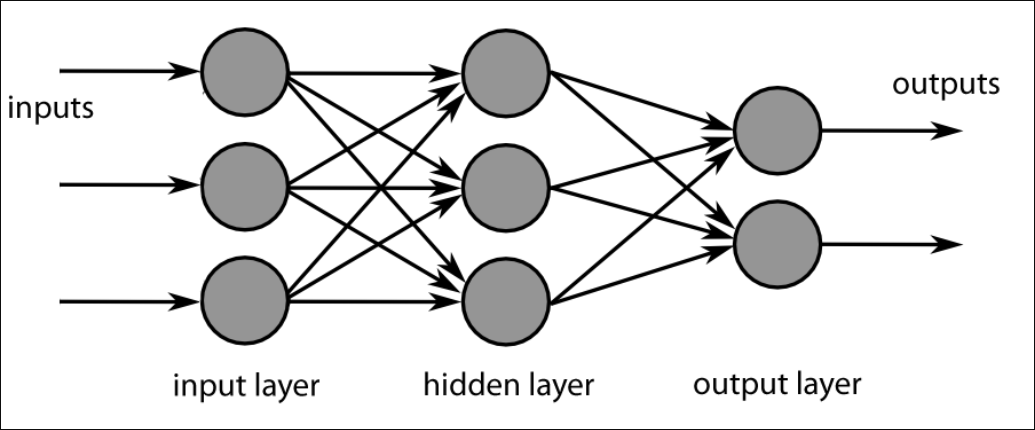
\includegraphics[width=.6\textwidth]{assets/rete-neur-visual.png}
    \end{center}
\end{note}
\begin{note}[Recurrent]
    Nelle reti \textbf{ricorrenti} sono previste \red{connessioni di feedback}, in genere verso neuroni dello stesso livello.
    Questo complica notevolmente il flusso delle informazioni e l'addestramento, richiedendo di considerare il comportamento in più istanti temporali, \textbf{unfolding in time}.
    \\
    D'altro canto queste reti sono più indicate per la gestione di \textbf{sequenze}, perché dotate di un \textbf{effetto memoria}, di breve termine, che al tempo $t$ rende disponibile l'informazione processata a $t-1$, $t-2$, etc.
    Un particolare tipo di rete ricorrente è \ac{lstm}.
\end{note}
% section Tipologie di Reti Neurali (end)
%
\section{Multilayer Perceptron}\label{sec:multilayer_perceptron} % (fold)
Il termine \textbf{perceptron} (percettrone) deriva dal modello di neurone proposto da Rosenblatt.
\\
Il percettrone utilizza una funzione di attivazione lineare a soglia.
Un singolo percettrone, o una rete di percettroni a due soli livelli (input e output), può essere addestrato con una semplice regola chiamata \textbf{delta rule} (ispirata alla regola di \textbf{Hebb}).
\begin{cimage}
    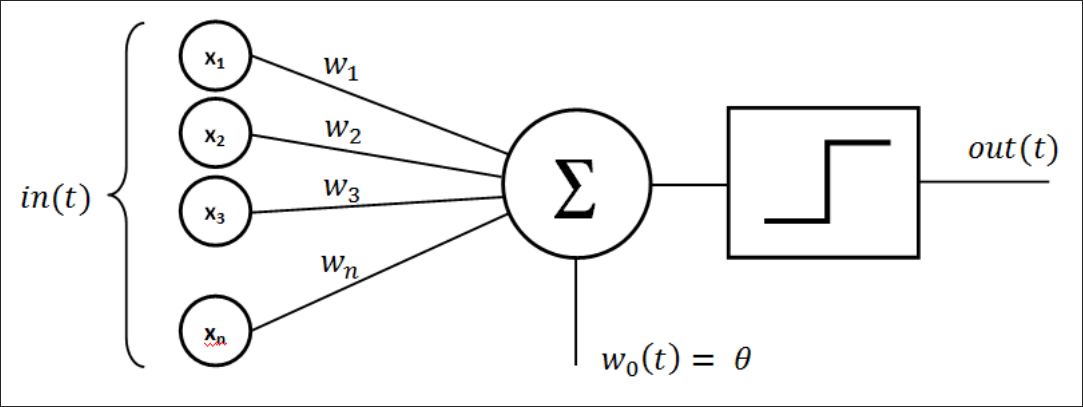
\includegraphics[width=.6\textwidth]{assets/mlp-visual.png}
\end{cimage}
Una rete a due livelli di percettroni lineari a soglia è in grado di apprendere solo mapping lineari e pertanto il numero di funzioni approssimabili è piuttosto limitato.
\begin{definition}{MLP}{}
    Un \textbf{\ac{mlp}} è una rete feedforward con almeno $3$ livelli (almeno $1$ nascosto) e con funzioni di attivazione non lineari.
\end{definition}
Un teorema noto come \textbf{universal approximation theorem} asserisce che ogni funzione continua che mappa intervalli di numeri reali su un intervallo di numeri reali può essere approssimata da un \ac{mlp} con un solo hidden layer.
\subsection{Forward Propagation}\label{sub:mlp_forward_propagation} % (fold)
Con \textbf{forward propagation} (o \red{inference}) si intende la propagazione dell'informazione in avanti: dal livello di input a quello di output.
Una volta addestrata, una rete neurale può semplicemente processare pattern attraverso \textbf{forward propagation}.
\begin{cimage}
    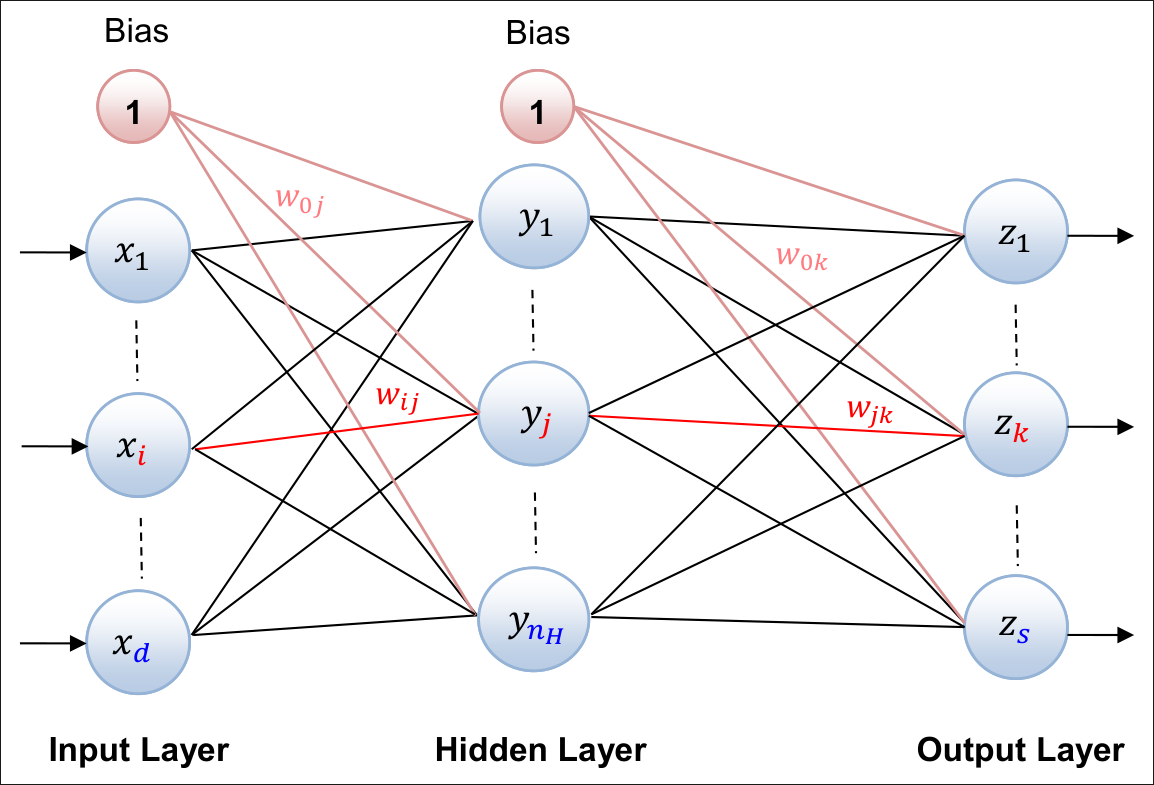
\includegraphics[width=.6\textwidth]{assets/rete-3-lvl-mlp.png}
    \caption{}\label{fig:rete-3-lvl-mlp}
\end{cimage}
In \cref{fig:rete-3-lvl-mlp} una rete a $3$ livelli $\pt{d:n_h:s}$: \red{input} $d$ neuroni, \red{livello nascosto} $n_h$ neuroni, \red{output} $s$ neuroni.
\\
Il numero totale di \textbf{pesi} (o parametri) è: $d \times n_h + n_h \times s + n_H + s$; dove gli ultimi due termini corrispondono ai pesi dei bias.
\\
Invece il $k$-esimo valore di output può essere calcolato come:
\begin{equation}
    \begin{aligned}\label{eq:forw-prop}
        z_k &= f\pt{\sum_{\for[j][][n_h]}w_{jk} \cdot y_j + w_{0k}} \\
            &= f\pt{\sum_{\for[j][][n_h]}w_{jk}\cdot f\pt{\sum_{\for[][][d]}{w_{ij}\cdot x_i + w_{0j}}} + w_{0k}}
    \end{aligned}
\end{equation}
\begin{cimage}
    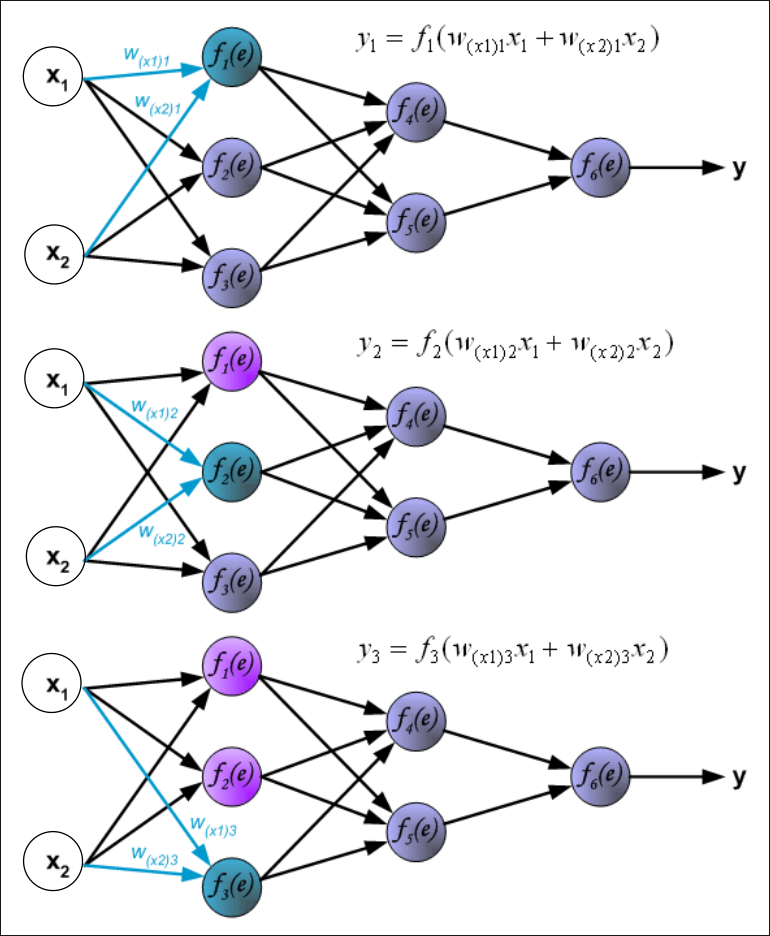
\includegraphics[width=.3\textwidth]{assets/forw-prop-visual.png}
\end{cimage}
%
% subsection Forward Propagation (end)
\subsection{Training}\label{sub:mlp_training} % (fold)
Fissata la topologia, l'addestramento di una rete neurale consiste nel \textbf{determinare il valore dei pesi} $w$ che determinano il \textbf{mapping desiderato} tra input e output.
\begin{quote}[Cosa si intende per mapping desiderato?]
    Se la rete neurale deve operare come un \link[chap:classificazione]{classificatore}, l'output desiderato è l'etichetta corretta della classe del pattern in input.
    Se la rete deve risolvere un problema di \link[chap:regressione]{regressione}, l'output desiderato è il valore corretto della variabile dipendente, in corrispondenza del valore della variabile indipendente fornita in input.
\end{quote}
Nel 1986 Rumelhart, Hinton e Williams hanno introdotto l'algoritmo di \textbf{Error Backpropagation} suscitando grande attenzione scientifica: l'algoritmo risolve il cosiddetto problema del \textbf{credit assignment}, ovvero quali pesi sono responsabili per gli errori.
\\
Matematicamente si tratta dell'applicazione della regola di \textbf{derivazione a catena}, idea che però per decenni nessuno aveva applicato con successo in questo contesto.
\begin{cimage}
    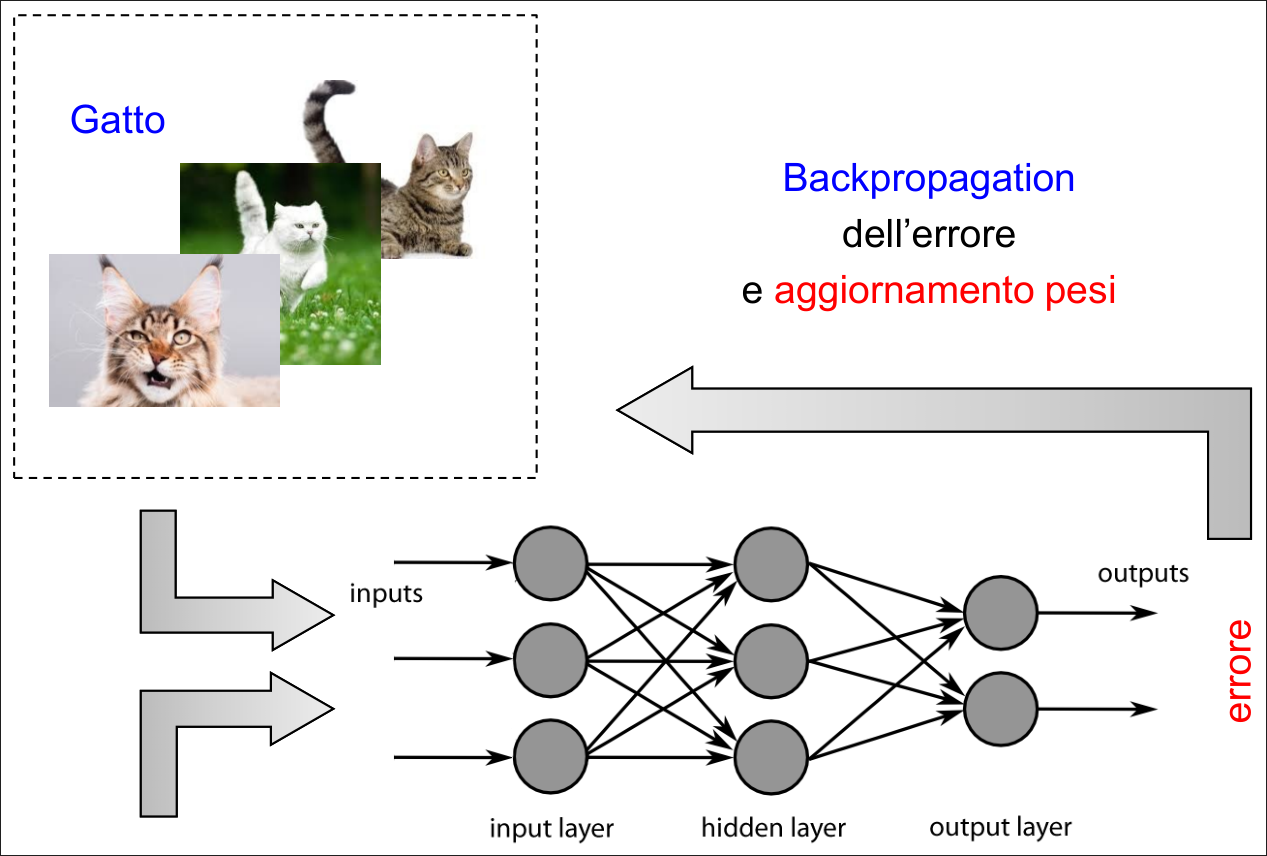
\includegraphics[width=.6\textwidth]{assets/mlp-train-visual.png}
\end{cimage}
% subsection Training (end)
%
\subsection{Backpropagation}\label{sub:backpropagation} % (fold)
Per gestire un problema di classificazione con $s$ classi e pattern $d$-dimensionali,si può utilizzare una rete \ac{mlp} con $d:n_H:s$ neuroni nei tre livelli.
Ovvero tanti neuroni di input quante sono le feature e tanti neuroni di output quante sono le classi.
$n_H$ è invece un \textbf{iperparametro}: un valore ragionevole è $n_H = 1 / 10^n$.
\emptyln{}
La \red{pre-normalizzazione} dei pattern di input, attraverso min-max scaling, standardization o whitening, favorisce la convergenza durante l'addestramento.
L'addestramento supervisionato avviene presentando alla rete pattern di cui è nota la classe e propagando (\link[sub:mlp_forward_propagation]{forward propagation}) gli input verso gli output attraverso l'\cref{eq:forw-prop}.
\\
Dato un pattern di training di classe $g$, il vettore di output desiderato $t$ (usando $\tanh$ come funzione di attivazione) assume la forma:
\[
    t = \ps{-1,\,-1,\,\dots,\,1,\,\dots,\,-1}
\]
La differenza tra l'output prodotto della rete e quello desiderato è l'errore della rete.
L'obiettivo dell'algoritmo di apprendimento è di \textbf{modificare i pesi della rete} in modo da \textbf{minimizzare l'errore medio sui pattern} del training set.
Prima dell'inizio dell'addestramento i pesi sono inizializzati con valori \red{random in range specifici}.
\emptyln{}
Siano:
\begin{itemize}
    \item $z = \ps{\vc{z_1}{z_s}}$ l'output prodotto dalla rete, tramite forward propagation, in corrispondenza del pattern $x = \ps{\vc{x_1}{x_d}}$ di classe $g$ fornito in input;
    \item $t = \ps{\vc{t_1}{t_2}}$ l'output desiderato, dove $t_i = 1$ per $i = g$, $t_i = -1$ altrimenti;
\end{itemize}
Scegliendo come \red{loss function} la \textbf{somma dei quadrati degli errori}, l'errore per il pattern $x$ è:
\[
    J\pt{w,x} \equiv \half\sum_{\for[c][][s]}\pt{t_c-z_c}^2
\]
che quantifica l'output prodotto per il pattern $x$ si discosta da quello desiderato.
\begin{note}
    \begin{itemize}
        \item la dipendenza dai pesi $w$ è implicita in $z$;
        \item l'errore $J\pt w$ sull'intero training set è la media di $J\pt{w,x}$ su tutti i pattern $x$ appartenenti al training set;
        \item la somma dei quadrati degli errori \red{non è una loss ottimale} per la classificazione;
    \end{itemize}
\end{note}
$J\pt w$ può essere ridotto modificando i pesi $w$ in direzione \textbf{opposta al gradiente} di $J$.
Infatti il vettore gradiente indica la direzione di maggior crescita di una funzione e muovendoci in direzione \red{opposta} si riduce al massimo l'errore.
\emptyln{}
Quando la minimizzazione dell'errore avviene attraverso passi in direzione opposta al gradiente l'algoritmo di \textbf{backpropagation} è denominato anche \textbf{gradient descent}.
Esistono anche tecniche di minimizzazione del secondo ordine che possono accelerare la convergenza.
\begin{cimage}
    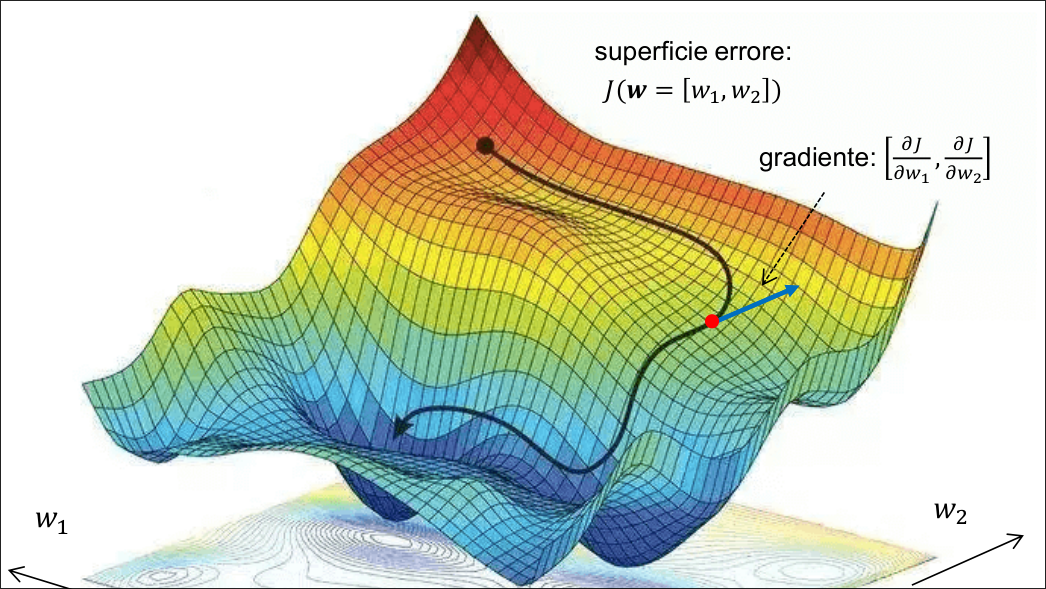
\includegraphics[width=.6\textwidth]{assets/backprop-grad-visual.png}
\end{cimage}
In seguito si considerano:
\begin{itemize}
    \item la modifica dei pesi $w_{jk}$ \textbf{hidden-output};
    \item la modifica dei pesi $w_{ij}$ \textbf{input-hidden};
\end{itemize}
%
\subsubsection{Modifica pesi hidden-output}\label{sec:bp_modifica_pesi_hidden_output} % (fold)
\begin{equation}
    \begin{aligned}
        \frac{\dd J}{\dd w_{jk}} &= \frac{\dd}{\dd w_{jk}}\pt{\half \sum_{\for[c][][s]} \pt{t_c-z_c}^2} \\
                                 &=\pt{t_k - z_k}\frac{\dd \pt{-z_k}}{\dd w_{jk}} \\
                                 &=\pt{t_k-z_k}\frac{\dd\pt{-\fx[net_k]}}{\dd w_{jk}} = -\pt{t_k-z_k}\cdot\frac{\fx[net_k]}{\dd net_k}\cdot\frac{\dd net_k}{\dd w_{jk}} \\
                                 &=-\pt{t_k-z_k}\cdot \dfx[net_k]\cdot\frac{\dd\sum_{\for[s]}w_{sk}\cdot y_s}{\dd w_{jk}} \\
                                 & = -\pt{t_k-z_k}\cdot\dfx[net_k]\cdot y_j
    \end{aligned}
\end{equation}
posto $\dt_k = \pt{t_k-z_k}\cdot \dfx[net_k]$, allora $\frac{\dd J}{\dd w_{jk}} = -\dt_k\cdot t_j$
\\
Pertanto il peso $w_{jk}$ può essere aggiornato come:
\begin{equation}\label{eq:bp-w-update}
    w_{jk} = w_{jk} + \eta \cdot \dt_k \cdot y_j
\end{equation}
dove $\eta$ è il \textbf{learning rate}.
\begin{note}
    Se si usano i \red{bias} il peso $w_{0k}$ si aggiorna ponendo $y_0 = 1$
\end{note}
% subsubsection BP: modifica pesi hidden-output (end)
\subsubsection{Modifica pesi input-hidden}\label{sec:bp_modifica_pesi_input_hidden} % (fold)
\begin{equation}
    \begin{aligned}
        \frac{\dd J}{\dd w_{ij}} &= \frac{\dd}{\dd w_{ij}}\pt{\half\sum_{\for[c][][s]}\pt{t_c-z_c}^2} = -\sum_{\for[c][][s]}\pt{t_c-z_c}\frac{\dd z_c}{\dd w_{ij}} \\
                                 &= -\sum_{\for[c][][s]}\pt{t_c-z_c}\frac{\dd z_c}{\dd net_c}\cdot\frac{\dd net_c}{\dd w_{ij}} = -\sum_{\for[c][][s]}\pt{t_c-z_c}\cdot\dfx[net_c]\cdot\frac{\dd net_c}{\dd w_{ij}} \\
    \end{aligned}
\end{equation}
con:
\begin{equation*}
    \begin{aligned}
        \frac{\dd net_c}{\dd w_{ij}} &= \frac{\dd}{\dd w_{ij}}\sum_{\for[r][][n_H]}w_{rc}\cdot y_r = \frac{\dd}{\dd w_{ij}} \sum_{\for[r][][n_H]}w_{rc}\cdot\dfx[net_r] \\
                                     &= \frac{\dd}{\dd w_{ij}}\pt{w_{jc}\cdot\fx[net_j]} = w_{jc}\frac{\dd \fx[net_j]}{\dd net_j}\cdot\frac{\dd net_j}{\dd w_{ij}} \\
                                     &= w_{jc} \cdot \dfx[net_j] \cdot \frac{\dd}{\dd w_{ij}} \sum_{\for[q][][d]}w_{qj}\cdot x_q = w_{jc} \cdot \dfx[net_j] \cdot x_i
    \end{aligned}
\end{equation*}
\begin{equation*}
    \frac{\dd J}{\dd w_{ij}} = -\sum_{\for[c][][s]}\dt_c \cdot w_{jc} \cdot \dfx[net_j]\cdot x_i = -x_i \cdot \dfx[net_j]\sum_{\for[c][][s]}w_{jc}\cdot\dt_c
\end{equation*}
Posto $\dt_j = \dfx[net_j]\cdot\sum_{\for[c][][s]}w_{jc}\cdot \dt_c$ allora $\frac{\dd J}{\dd w_{ij}} = -\dt_j \cdot x_i$
\\
Pertanto il peso $w_{ij}$ può essere aggiornato come:
\begin{equation}\label{eq:bp-input-hidden}
    w_{ij} = w_{ij} + \eta \cdot \dt_j \cdot x_i
\end{equation}
\begin{note}
    Se si usano i \red{bias} il peso $w_{0j}$ si aggiorna ponendo $x_0 = 1$
\end{note}
%
% subsubsection BP: modifica pesi input-hidden (end)
\subsubsection{BP: Algoritmo}\label{sec:bp_algoritmo} % (fold)
Nella versione \red{online} i pattern del training set sono presentati sequenzialmente e i pesi sono aggiornati dopo la presentazione di ogni pattern:
\begin{cimage}
    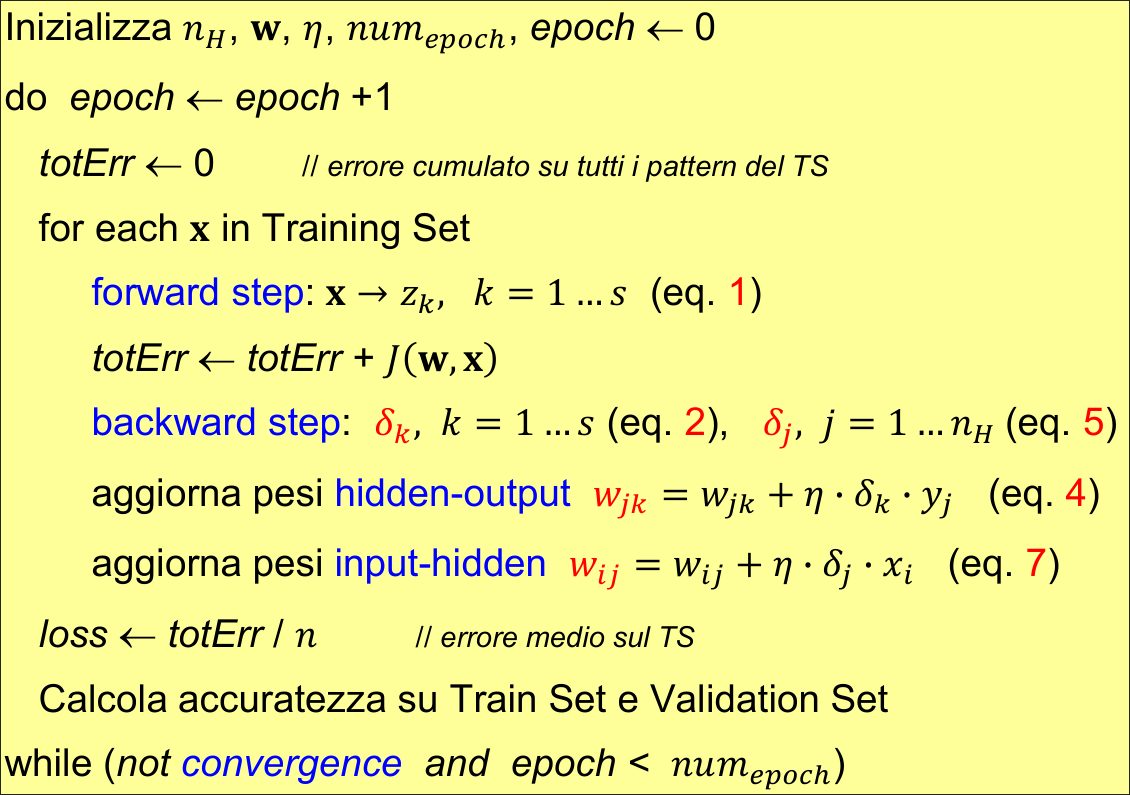
\includegraphics[width=.8\textwidth]{assets/bp-algo-online.png}
\end{cimage}
\begin{note}
    La \link[sub:convergenza]{convergenza} si valuta monitorando l'andamento del loss e l'accuratezza sul validation set
\end{note}
La versione online richiede l'aggiornamento dei pesi a seguito della presentazione di ogni pattern: problemi di \red{efficienza} e \red{robustezza}.
% subsubsection BP: Algoritmo (end)
% subsection Backpropagation (end)
%
\subsection{Stochastic Gradient Descent}\label{sub:stochastic_gradient_descent} % (fold)
È l'approccio più utilizzato per implementare backpropagation:
\begin{itemize}
    \item a ogni epoca, gli $n$ pattern del training set sono \red{ordinati} in modo \red{casuale} e poi suddivisi, considerandoli sequenzialmente, in gruppi (denominati \textbf{mini-batch}) di uguale dimensione $size_{mb}$:
        \begin{itemize}
            \item se $size_{mb} = 1 \rightarrow$ <<stochastic>> online;
            \item se $size_{mb} = n \rightarrow$ <<full>> batch;
        \end{itemize}
    \item i valori del \textbf{gradiente} sono algebricamente accumulati in variabili temporanee; l'aggiornamento dei pesi avviene solo quando tutti i pattern di un mini-batch sono stati processati;
\end{itemize}
\begin{cimage}
    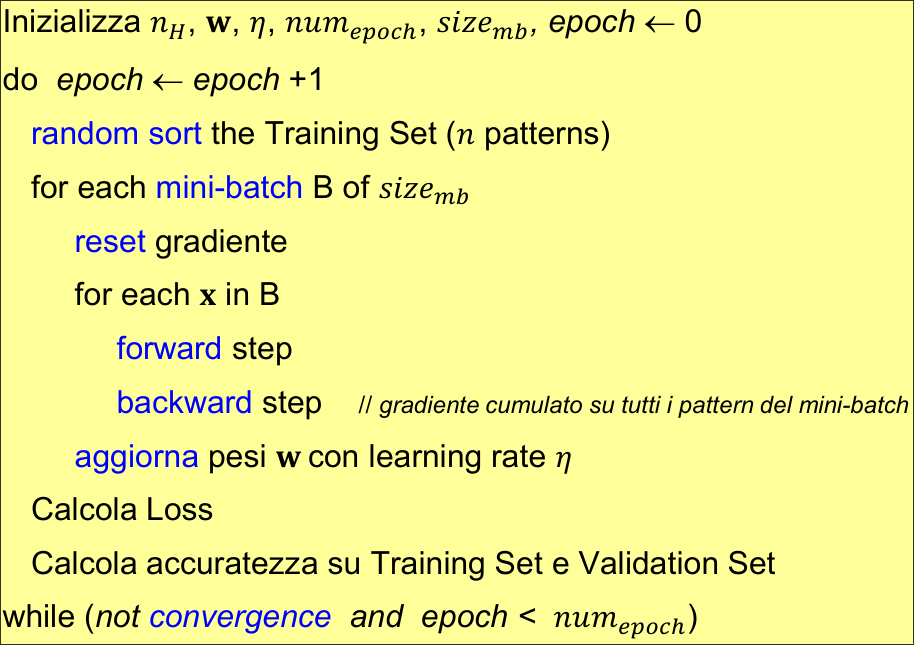
\includegraphics[width=.8\textwidth]{assets/stoc-grad-desc-algo.png}
\end{cimage}
%
\subsubsection{Terminologia (SGD)}\label{sec:terminologia_sgd_} % (fold)
Per \red{epoca} si intende la presentazione (1 volta) alla rete di tutti i pattern del training set.
\\
Per \red{iterazione} (iteration) si intende la presentazione (1 volta) dei pattern costituenti un mini-batch e il conseguentemente aggiornamento dei pesi.
\begin{quote}
    $n/size_{mb}$ è il numero di iterazioni per epoca. Se non è un valore intero all'ultima iterazione si processano meno pattern
\end{quote}
Invece di $num_{epoch}$ e $size_{mb}$ alcuni tool \textbf{richiedono in input il numero totale di iterazioni} $num_{iter}$ e $size_{mb}$; in questo caso il numero di epoche, non necessariamente intero, è:
\[
    num_{epoch} = \frac{num_{iter}\cdot size_{mb}}{n}
\]
\begin{note}[Tarare il mini-batch size]
    Definire il valore ottimale di $size_{mb}$ non è banale. 
    Se consideriamo la sola \red{efficienza}:
    \begin{itemize}
        \item $size_{mb}$ maggiori aumentano velocità del training: meno aggiornamenti del gradiente e processing più efficiente di mini-batch grandi;
        \item in modelli di più grandi dimensioni $size_{mb}$ è limitato dalla memoria disponibile nella GPU;
    \end{itemize}
    Relativamente alla \red{generalizzazione} però:
    \begin{itemize}
        \item si è osservato che i modelli generalizzano maggiormente quando convergono a \red{flat minima} non \red{sharp};
        \item mini-batch piccoli o di medie dimensioni sono più esplorativi e meno attratti da sharp minima, da cui con large mini-batch è difficile uscire;
    \end{itemize}
    $size_{mb}$ e il learning rate $\eta$ \red{non sono indipendenti}:
    \begin{itemize}
        \item in genere con mini-batch più grandi si può usare un learning rate più aggressivo grazie a un effetto <<media>> più forte nelle correzioni;
        \item alcuni autori propongono \textbf{aumento lineare} di $\eta$ all'aumentare di $size_{mb}$;
    \end{itemize}
\end{note}
% subsubsection Terminologia (SGD) (end)
% subsection Stochastic Gradient Descent (end)
% section Multilayer Perceptron (end)
%
\section{Approfondimenti}\label{sec:approfondimenti} % (fold)
\subsection{SoftMax: Output Probabilistico}\label{sub:softmax} % (fold)
Se nel livello di output si utilizza come funzione di attivazione:
\begin{itemize}
    \item $\tanh$: i valori di uscita sono nell'intervallo $\itc{-1,\,1}$, e quindi non sono probabilità;
    \item \link[par:sigmoid]{sigmoid}: i valori di uscita sono compresi nell'intervallo $\itc{0,\,1}$, ma non abbiamo nessuna garanzia che la somma sui neuroni di uscita sia $1$ (requisito fondamentale affinché si possano interpretare come distribuzione probabilistica):
        \[
            \sum_{\for[c][][s]}{z_c \ne 1}
        \]
\end{itemize}
Quando una rete neurale è utilizzata come \red{classificatore multi-classe}, l'impiego della funzione di attivazione \textbf{softmax} consente di trasformare i valori di \red{net} prodotti dall'ultimo livello della rete in probabilità delle classi:
\begin{itemize}
    \item il livello di attivazione $net_k$ dei singoli neuroni dell'ultimo livello si calcola nel modo consueto, ma come \red{funzione di attivazione} per il neurone $k$-esimo si utilizza:
        \[
            z_k = \frac{e^{net_k}}{\sum_{\for[c][][s]}e^{net_c}}
        \]
    \item i valori $z_k$ prodotti possono essere \textbf{interpretati come la probabilità delle classi}: appartengono a $\itc{0,\,1}$ e la loro somma è $1$;
    \item l'esponenziale, utile nella combinazione con Cross Entropy Loss, interpreta i valori $net$ come \textbf{unnormalized log probabilities} delle classi;
\end{itemize}
% subsection SoftMax: Output Probabilistico (end)
%
\subsection{Cross-Entropy Loss}\label{sub:cross_entropy_loss} % (fold)
Per un problema di \textbf{classificazione multi-classe} si consiglia l'utilizzo di \textbf{Cross-Entropy} come \red{loss function}.
\begin{definition}{Cross-Entropy Loss}{}
    La cross-entropy tra due distribuzioni discrete $p$ e $q$ (che fissata $p$ misura quanto $p$ differisce da $p$) è definita da:
    \[
        H\pt{p,\,q} = -\sum_v{p\pt v \cdot \log{\pt{q\pt v}}}
    \]
    Nell'impiego come loss function: $p$ (fissato) è il vettore \red{target}, mentre $q$ il vettore di \red{output} della rete.
\end{definition}
Il valore minimo di $H$, sempre $\ge 0$, si ha quando il vettore target coincide con l'output.
%
\subsubsection{One-hot targets}\label{sec:one_hot_targets} % (fold)
Quando il target vector per $x$ assume la forma \red{one-hot}, tutti $0$ tranne $1$ per la classe corretta $g$:
\[
    t = \ps{0,\,0,\,\dots,\,1,\,\dots,\,0}
\]
allora:
\[
    J\pt{w,\,x} \equiv H\pt{t,\,z} = -\log{\pt{z_g}}
\]
Se $z_g$ è ottenuta con funzione di attivazione \red{softmax}, allora:
\[
    J\pt{w,\,x} = -\log{\pt{\frac{e^{net_g}}{\sum_{\for[c][][s]}{e^{net_c}}}} = -net^g + \log{\sum_{\for[c][][s]}e^{net_c}}}
\]
% subsubsection One-hot targets (end)
%
\subsubsection{Loss Function per Regressione}\label{sec:loss_function_per_regressione} % (fold)
Consideriamo un problema di regressione dove sia la variabile indipendente (input) che quella dipendente (output) sono vettori.
\begin{quote}
    \begin{itemize}
        \item Utilizzando la terminologia introdotta per la regressione si affronta un problema di \red{multivariate multiple regression};
        \item La rete neurale è in grado di trovare un mapping non lineare tra input e output, pertanto il termine \link[sec:lineare]{linear} non si applica;
    \end{itemize}
\end{quote}
Se l'output assume valori \red{reali non limitati} si consiglia di non utilizzare funzioni di attivazione nel livello finale: i target vector $t$ non sono soggetti a vincoli.
\[
    t = \ps{\vc{t_1}{t_n}}
\]
In ogni caso è consigliabile, per maggiore stabilità riscalare l'output nel range $\itc{0,\,1}$.
\begin{quote}
    Come \red{loss function} si può usare una qualsiasi fra: \link[def:rmse]{\ac{mse}}, \link[def:mae]{\ac{mae}}, \link[def:mape]{\ac{mape}}
\end{quote}
% subsubsection Loss Function per Regressione (end)
% subsection Cross-Entropy Loss (end)
%
\subsection{Inizializzazione dei pesi}\label{sub:inizializzazione_dei_pesi} % (fold)
L'inizializzazione random dei pesi in un \red{range ottimale} è molto importante per la convergenza della rete.
\\
La <<vecchia>> inizializzazione con \textbf{distribuzione normale a media 0 e deviazione standard 1}, tende a produrre una varianza degli output di un livello maggiore di quella degli input.
Ciò combinato con funzioni di attivazione \red{saturanti} (come \link[par:sigmoid]{sigmoid} e \red{tanh}) può portare a correzioni quasi nulle del gradiente e quindi la rete tende a non convergere.
\emptyln{}
\begin{definition}{Inizializzazione Xavier}{}
    Per mantenere la varianza di output simile a quella di input si possono inizializzare i pesi: con distribuzione normale a media $0$ e deviazione standard:
    \[
        \si = \sqrt{\frac{1}{fan_{avg}}}
    \]
    dove $fan_{avg}$ è la media tra il numero di input $fan_{in}$ e output $fan_{out}$ del livello.
    \\
    Con distribuzione uniforme in: $\itc{-\sqrt{\dfrac{3}{fan_{avg}}},\,+\sqrt{\dfrac{3}{fan_{avg}}}}$
\end{definition}
In combinazione con la funzione di attivazione \red{Relu} (funzione non saturante), l'\textbf{inizializzazione He} è utilizzata di default, dove:
\[
    \si = \sqrt{\frac{2}{fan_{in}}}
\]
% subsection Inizializzazione dei pesi (end)
%
\subsection{Regolarizzazione}\label{sub:regolarizzazione} % (fold)
Per ridurre il rischio di \red{overfitting} del training set da parte di una rete neurale con \red{molti parametri}, si possono utilizzare tecniche di \red{regolarizzazione}.
\\
La regolarizzazione è importante quando il training set non ha grandi dimensioni rispetto alla capacità del modello:
reti neurali i cui pesi, o parte di essi, assumono \textbf{valori piccoli} producono output più regolare e stabile, portando spesso a migliore \textbf{generalizzazione}.
\\
Per spingere la rete ad adottare pesi di valore piccolo si può aggiungere un termine di \textbf{regolarizzazione alla loss}.
Ad esempio nel caso di Cross-Entropy Loss:
\[
    J_{tot} = J_{Cross-Entropy} + J_{reg}
\]
Nella regolarizzazione \textbf{L2} il termine aggiunto corrisponde alla somma dei quadrati di tutti i pesi della rete:
\[
    J_{reg} = \half \lb\sum_iw_i^2
\]
Nella regolarizzazione \textbf{L1} si utilizza il valore assoluto:
\[
    J_{reg} = \lb\sum_i\ab{w_i}
\]
In entrambi i casi il parametri $\lb$ regola la forza della regolarizzazione.
\begin{note}
    L1 può avere un effetto \textbf{sparsificante}, ovvero portare numerosi pesi a $0$, maggiore di L2.
    Infatti quando i pesi assumono valori vicini allo zero il calcolo del quadrato in L2 ha l'effetto di ridurre eccessivamente i correttivi ai pesi rendendo difficile azzerarli.
\end{note}
%
\subsubsection{Weight Decay}\label{sec:weight_decay} % (fold)
Consideriamo la regolarizzazione L2: il gradiente della $J_{tot}$ rispetto a uno dei parametri della rete corrisponde alla somma del gradiente di $J_{Cross-Entropy}$ e del gradiente $J_{reg}$.
Quest'ultimo vale:
\[
    \frac{\dd J_{reg}}{\dd w_k} = \frac{\dd}{\dd w_k}\pt{\half\lb \sum_{w_i^2}} = \lb \cdot w_k
\]
pertanto l'aggiornamento dei pesi a seguito di backpropagation include un ulteriore termine denominato \textbf{weight decay} che ha l'effetto di \red{tirarlo verso} lo $0$.
% subsubsection Weight Decay (end)
\begin{example}{}{}
    Considerando l'aggiornamento dei pesi di \link[sub:stochastic_gradient_descent]{SGD}:
    \[
        w_k = w_k - \eta \cdot \frac{\dd J_{Cross-Entropy}}{\dd w_k}
    \]
    diventa:
    \[
        w_k = w_k - \eta \pt{\frac{\dd J_{Cross-Entropy}}{\dd w_k} + \lb \cdot w_k}
    \]
\end{example}
% subsection Regolarizzazione (end)
%
\subsection{Tarare il Learning Rate}\label{sub:tarare_il_learning_rate} % (fold)
Tarare il learning rate $\eta$ in modo ottimale è molto importante:
\begin{itemize}
    \item se \textbf{troppo piccolo} la convergenza è lenta ed è più facile rimanere bloccati in \red{minimi locali};
    \item se troppo grande oscillazione e/o divergenza;
\end{itemize}
\begin{cimage}
    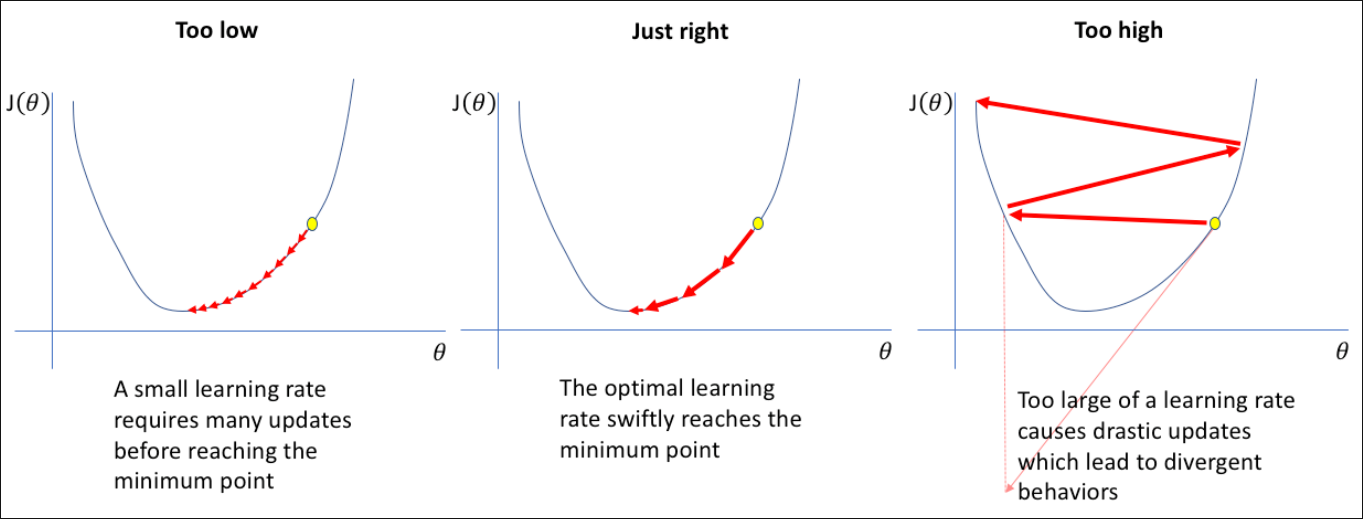
\includegraphics[width=.8\textwidth]{assets/tarare-learning-rate.png}
\end{cimage}
Il valore ottimale cambia a seconda dell'architettura della rete, della loss function, del mini-batch, etc.
\\
Tecniche di \textbf{scheduling} di learning rate e ottimizzatori con learning rate \textbf{adattivo} possono essere di aiuto.
\begin{warning}
    Il fatto che la loss diminuisca senza oscillare, non significa che il valore sia ottimale (specialmente nel tuning di reti pre-addestrate): \textbf{monitorare l'accuratezza sul validation set}.
\end{warning}
% subsection Tarate il Learning Rate (end)
%
\subsection{Momentum}\label{sub:momentum} % (fold)
\link[sub:stochastic_gradient_descent]{SGD} con mini-batch può determinare una discesa del gradiente a \textbf{zig-zag} che rallenta la convergenza e la rende meno stabile: la discesa del gradiente può essere vista come la traiettoria di una biglia che rotola su una superficie sconnessa.
Attratta dalla forza di gravità la biglia cerca di portarsi sul punto più basso.
\\
Nella fisica il \textbf{momento} conferisce alla biglia un moto privo di oscillazioni e cambi di direzione repentini.
Inoltre l'inerzia accumulata consente di superare piccoli avvallamenti (minimi locali).
\emptyln{}
In \link[sub:stochastic_gradient_descent]{SGD} per evitare oscillazioni si può emulare il comportamento fisico: si tiene traccia dell'ultimo aggiornamento $\Dt w_k$ di ogni parametro $w_k$, e il \textbf{nuovo aggiornamento} è calcolato come \textbf{combinazione lineare} del precedente aggiornamento (che conferisce stabilità) e del gradiente attuale $\frac{\dd J}{\dd w_i}$ (che corregge la direzione):
\[
    \Dt w_k = \mu \cdot \Dt w_k - \eta \frac{\dd J_{tot}}{\dd w_k}
\]
\begin{cimage}
    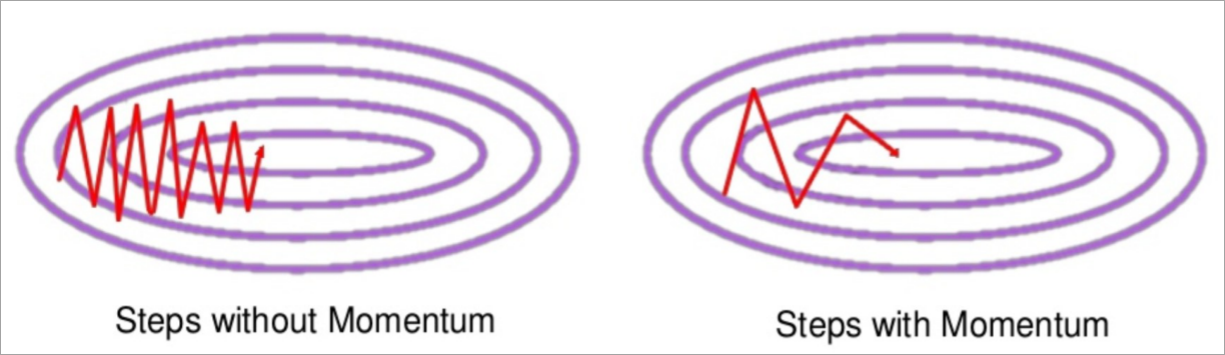
\includegraphics[width=.8\textwidth]{assets/momentum-visual.png}
\end{cimage}
Valore tipico del parametro $\mu = 0.9$
% subsection Momentum (end)
%
\subsection{Learning Rate adattivo}\label{sub:learning_rate_adattivo} % (fold)
Oltre a \link[sub:momentum]{Momentum} esistono altri ottimizzatori per l'aggiornamento dei pesi che possono accelerare la convergenza nella discesa del gradiente:
\begin{itemize}
    \item \ac{nag};
    \item \ac{adagrad};
    \item \red{Adadelta};
    \item \red{RMSProp};
    \item \red{Adam} e \red{AdamW};
\end{itemize}
La maggior parte di adatta il learning rate $\eta$ a ogni specifico parametro: passi di discesa più lunghi lungo le direzioni in cui il gradiente varia poco.
È necessario mantenere statistiche (parametro per parametro) sulla variazione del gradiente.
\red{Adam} è considerato lo stato dell'arte, anche se non sempre fornisce risultati del più classico \link[sub:stochastic_gradient_descent]{SGD} con \link[sub:momentum]{momentum}.
\begin{cimage}
    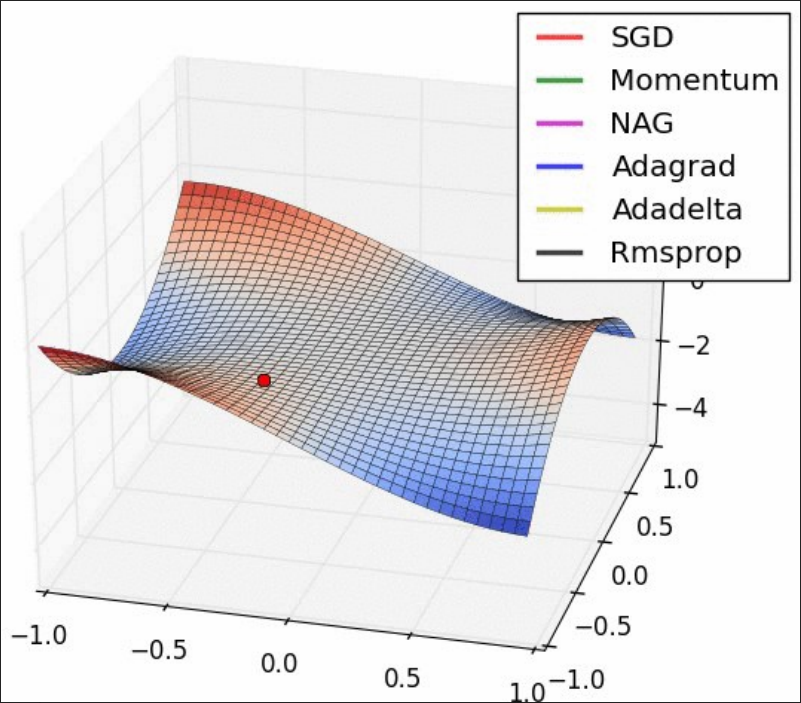
\includegraphics[width=.8\textwidth]{assets/learn-rate-adatt-visual.png}
\end{cimage}
% subsection Learning Rate adattivo (end)
\begin{note}[La rete non converge: check list]
    Nel seguito alcune cose da verificare quando la convergenza sul training set non parte (la rete sembra bloccata).
    \begin{itemize}
        \item Gli \red{input} sono stati \textbf{normalizzati} (min-max, standard scaling)?
        \item I \red{pesi} sono stati \textbf{inizializzati} random in range ragionevoli (Xavier, He)?
            Altrimenti potremmo essere in zona saturazione da cui non è possibile uscire;
        \item I pattern delle diverse classi sono stati \red{mescolati} random all'interno dei mini-batch?
        \item Le \red{etichette} sono nel \textbf{formato giusto} (interi sparsi, one-hot vectors, float per regressione)?
        \item La \red{loss function} è corretta e adeguata al tipo di label fornite (attenzione alla differenza tra label sparse e vettori one-hot)?
        \item La \red{funzione di attivazione} all'ultimo livello è corretta (sigmoid per binary classification, softmax per Cross-Entropy multiclasse, null per regressione)?
        \item Il \red{learning rate} è adeguato?
    \end{itemize}
\end{note}
% section Approfondimenti (end)
% chapter Reti Neurali (end)
